\documentclass[runningheads,a4paper]{llncs}

\setcounter{tocdepth}{3}
\usepackage{natbib}
\usepackage[english]{babel}
\usepackage{graphicx}
\usepackage{subcaption}
\usepackage{algorithm}
\usepackage{algpseudocode}
\usepackage{amsmath, amssymb, mathtools, amsthm}
\usepackage{hyperref}
\usepackage{url}
\usepackage[pages=some]{background}
\usepackage[margin=2.8cm]{geometry}
\usepackage{lipsum}
\graphicspath{{figures/}}
\definecolor{MVA}{HTML}{652475}

\newcommand\BackGroundImage[1]{%
\BgThispage
\backgroundsetup{
    scale=1,angle=0,position={current page.north}, hshift=-7.5cm, 
    vshift=-1.5cm, opacity=1,
    contents={%
    \includegraphics[width=5cm]{#1}
}}}

\newcommand{\R}{\mathbb{R}}
\newcommand{\E}{\mathbb{E}}
\renewcommand{\S}{\mathbb{S}}
\newcommand{\X}{\mathcal{X}}
\newcommand{\A}{\mathcal{A}}
\renewcommand{\P}{\mathcal{P}}
\newcommand{\KL}{\mathrm{KL}}
\newcommand{\W}{\mathbb{W}}
\renewcommand{\H}{\mathcal{H}}
\renewcommand{\S}{\mathbb{S}}
\newcommand{\diff}[2]{\frac{\partial #1}{\partial #2}}
\renewcommand{\d}{\: \mathrm{d}}
\newcommand{\Stein}{I_{Stein}(\mu | \pi)}
\DeclarePairedDelimiter{\norm}{\|}{\|}
\DeclarePairedDelimiter{\pare}{(}{)}
\DeclarePairedDelimiter{\bra}{\{}{\}}
\DeclarePairedDelimiter{\sq}{[}{]}
\DeclarePairedDelimiter{\sca}{\langle}{\rangle}
\renewcommand\qedsymbol{$\blacksquare$}

\begin{document} 

\mainmatter
\titlerunning{Stein Variational Gradient Descent: Main ideas}
\title{Stein Variational Gradient Descent: Main ideas}

\author{Gaëtan Serré and Perceval Beja-Battais}
\authorrunning{Serré and Beja-Battais}

\institute{École Normale Supérieure Paris-Saclay\\
Master Mathématiques, Vision, Apprentissage\\
\{gaetan.serre, perceval.beja-battais\}@ens-paris-saclay.fr}

\toctitle{Stein Variational Gradient Descent: Main ideas}
\tocauthor{Gaëtan Serré and Perceval Beja-Battais}
\maketitle

\BackGroundImage{MVA.pdf}

\section{Introduction}
In this paper we will contextualize and describe the article \cite{main-paper}. The goal is to be able to sample from an unknown distribution $\pi$ thanks to an iterative procedure that is called Stein Variational Gradient Descent (SVGD). It was first introduced by \cite{Original-SVGD}. Starting from an initial distribution $\mu_0$, this algorithm can be seen as a gradient descent in the Wasserstein space of distributions $\P_2(\X)$, with $\X \in \R^d$.
{\bf TODO METTRE NOS CONTRIBS}

\section{SVGD Context (\cite{Original-SVGD})}
In all what follows, $\X = \R^d$. \newline
We fix here $\pi$ an objective distributions from which we want to sample, and an initial distribution from which we know how to sample $\mu_0$. 
\subsection{Notations}
We will denote as earlier by $\P_2(\X)$ the Wasserstein space of distributions i.e. the set of distributions such that $\int ||x||^2 d\mu(x) < \infty$. We assume the objective distribution $\pi$ lives in $\P_2(\X)$, and define the Kullback-Liebler divergence between $\pi_1$ and $\pi_2$ by
$$\KL(\pi_1||\pi_2) := \E_{\pi_1} [\log \pi_1(x)] - \E_{\pi_1}[\log \pi_2(x)]$$ \newline
Let $\A_\pi$ the Stein Operator defined by $\forall \phi \in \H, \forall x \in \X, \A_\pi \phi(x) = \nabla \log \pi(x) \phi(x)^\top + \nabla\cdot \phi(x)$, for some $\H$ we will precise later on. \newline
We define the Stein class of $\pi$ the subset of functions $\phi$ such that $\lim_{||x||\longrightarrow \infty} \phi(x)\pi(x) = 0$. Note that for every function in the Stein class of $\pi$, we have \begin{equation}
  \E_{x \sim \pi}[\A_\pi \phi (x)] = 0
  \label{eq:stein_id}
\end{equation}
(See \ref{proof:stein_id} for the proof)\newline
Also, we define the pushforward measure of $\mu$ by $T:\R^d \longrightarrow \R^d$ by $\int \phi(T(x)) d\mu(x) = \int \phi(x) dT_\#\mu(x)$ for any bounded and measurable function $\phi$. \newline
The gradient of $\KL(\cdot||\pi)$ at $\mu$ in $\P_2(\X)$ is given by $\nabla_{W_2}\KL(\mu||\pi) = \nabla \log(\frac{\mu}{\pi})$. The idea behind SVGD is to iteratively follow the descent direction given by $\nabla_{W_2} \KL (\cdot||\pi)$. \newline
Finally, for $\phi : \R^d \longrightarrow \R^d$, we denote by $||\phi||_{op}$ the operator norm. \newline

\subsection{Context}
Let $\mu \in \P_2(\X)$. Given a smooth function $\phi = [\phi_1,...,\phi_d]^\top$, a small perturbation of $\mu$ in the direction of $\phi$ is given by 
\begin{equation}
    \mu_{[T]} = \mu_\#(I+\gamma \phi)
\end{equation}
for a small $\gamma > 0$. \newline
Recall that $\E_{x \sim \mu}[\A_\pi \phi (x)] = \int_\X \pare*{ \nabla \log \pi(x)^\top \phi(x) + \nabla \cdot \phi(x) } \mu(x) \d x$. As soon as $\mu$ is not in the Stein class of $\pi$, one can show that $\E_{x \sim \mu}[\A_\pi \phi (x)] > 0$, increasing w.r.t. the difference between $\mu$ and $\pi$ (Proof here: \ref{proof:Esp_distance}).. \newline
Therefore, the problem we want to solve is to find
\begin{equation}
  \mu^* = \arg\min_{\mu} \: \S(\mu, \pi) =
    \arg\min_{\mu} \: \max_{\phi \in \H} \bra*{ \E_{x \sim \mu}[\A_\pi \phi (x)] },
  \label{eq:stein_obj}
\end{equation}
for a certain class $\H$ of functionals. A question now raises: how to choose $\H$?
\subsubsection{Choice of $\H$}\label{sec:RKHS}
In all papers, $\H$ is chosen as the product RKHS of $\X$. We will quickly explain here why so. \newline
Let $\H_0$ be a RKHS with a kernel $k(x, x')$ in the Stein class of $\pi$.
Let $\H = (\H^{(1)}_0, \dots, \H^{(d)}_0)$. The KSD maximizes $\phi$ in the unit ball of $\H$.
The objective in (\ref{eq:stein_obj}) is then:
\begin{equation}
  \S(\mu, \pi) =
    \max_{\phi \in \H} \bra*{ \E_{x \sim \mu}[\A_\pi \phi (x)], \; s.t. \; \|\phi\|_{\H} \leq 1 }.
  \label{eq:stein_ksd_obj}
\end{equation}
Within this framework, one can show that the optimal solution of (\ref{eq:stein_ksd_obj})
is given by:
\begin{equation}
  \phi(x) = \frac{\phi^*(x)}{\|\phi^*\|_{\H}}
    \text{ , where } \phi^*(.) = \E_{x \sim \mu}\sq*{ \A_\pi \otimes k(x, \cdot) }
                               = \int_\X (k(x, \cdot) \nabla \log \pi(x) + \nabla k(x, \cdot)) \d \mu(x),
  \label{eq:stein_ksd_sol}        
\end{equation}
where $\A_\pi \otimes f(x) =  f(x) \nabla \log \pi(x) + \nabla f(x)$, is a variant of Stein operator. We also know that $\phi^*$ is in the Stein class of $\pi$ as $k$ is.
Moreover, $\S(\mu, \pi) = \|\phi^*\|_\H$. (Complete proof in \ref{proof:KSD})
\subsubsection{Return to the problem}
For $\gamma < \frac{1}{||\phi||_{op}}$, $(I+\gamma \phi)$ is locally one-to-one. We then have that $$\nabla_\gamma \KL(T_\#\mu||\pi)|_{\gamma = 0} = - \E_{x\sim \pi}[\A_\pi \phi(x)]$$ 
Considering all descent directions on the ball $\{\phi\in \H, ||\phi||^2_{op} \leq \S(\mu,\pi)\}$, the one we will keep for our gradient descent is the one minimizing the gradient of $\KL$, which writes $\phi^*$ as showed just earlier. \newline
The Stein Variational Gradient Descent (SVGD) algorithm consists
in an iterative procedure where one apply successive transformations
to an initial density $\mu_0$ following
the trajectory $\phi^*$ that minimizes the gradient of the Kullback-Leibler divergence:
\begin{equation}
  \mu_{n+1} = \pare*{ I + \gamma \phi^* }_\# \mu_n
  \label{eq:mu-n}
\end{equation}

%%%%%% A continuer : $$ \E_{x\sim \pi} [k(x, ·)\nabla x \log \pi(x) + \nabla xk(x, ·)] $$

\section{Non-asymptotic analysis of SVGD}
In their paper (\cite{main-paper}), under assumptions, the authors provide
an exponential convergence rate for continuous time SVGD, and
a convergence result between SVGD in the infinite particle setting
and in the finite particle setting.
This last result is very important as the latter
setting is the one used in practice
when implementing the SVGD algorithm and allows to
make a link between the implementation and the theoretical
results.
They also reprove a descent lemma for discrete time SVGD, originally
proved in 2017 (\cite{SVGD-flow}), using the Wassertein gradient
flow of the $\KL$ divergence.


\subsection{Optimal transport reminders}
Before going further, we will recall some notions of optimal transport
that the authors used throughout their paper.\\

\begin{definition}[Wasserstein distance]
  Let $\mu$ and $\nu$ be two probability measures on $\X$ and
  $$
    \Gamma (\mu, \nu) = \bra*{\gamma : \int_\X \gamma(x, y) \d y = \mu(x)
    \land \int_\X \gamma(x, y) \d x = \nu(y)}.
  $$
  The $p$-Wasserstein distance between $\mu$ and $\nu$ is defined by
  $$
    \W_p(\mu, \nu) = \inf_{\gamma \in \Gamma(\mu, \nu)} \int_\X \int_\X
    \norm*{x-y}^p \gamma(x, y) \d x \d y.
  $$
  This define a distance on the space of probability measures as it is
  positive, symmetric, $0$ if and only if $\mu = \nu$ and satisfies
  the triangle inequality.
\end{definition}

\begin{definition}[Continuity equation \cite{villani2003}]\label{def:continuity-equation}
  Let $\X$ be $\R^d$ and $(T_t)_{0 \leq t}$ a measurable map from $\X$ to $\X$
  such that $T_t = I + \phi(t)$.
  Let $v_t$ be the velocity field associated 
  with the trajectories $T_t$. Let $\mu_0 \in \P_2(\X)$
  and $\mu_{t+1} = T_t \# \mu_t$. Then, $\mu_t$ is the unique solution
  of the following continuity equation:
  $$
  \begin{cases}
    \diff{\mu_t}{t} + \nabla \cdot (v_t \mu_t) = 0 \\
    v_t = \phi(t).
  \end{cases}
  $$
  
\end{definition}

\subsection{RKHS operators}
In the entire paper, the authors let $\X$ be $\R^d$. They defined
the RKHS $\H$ and $\H_0$ on real-valued function of $\X$ the same way as in
Section~\ref{sec:RKHS}

\noindent
They start by defining operators on the RKHS.
\begin{definition}
  Let $S_\mu : L_2(\mu) \to \H$ be the operator defined by:
  $$
  S_\mu f = \int_\X k(x, \cdot) f(x) \d \mu(x).
  $$
  They also make the assumption that $\int_\X k(x, x) \d \mu(x) < \infty$,
  $\forall \mu \in \P_2(\X)$, which implies $\H \subset L^2(\mu)$
  (proof in \ref{pro:H-L2}).
\label{def:S-mu}
\end{definition}
They also defined the inclusion $\iota : L^2(\mu) \to \H$ and
its adjoint $\iota^* : \H \to L^2(\mu) = S_\mu$. Finally, they defined
$P_\mu = \iota S_\mu$. Thanks to these operators, we now have that:
$$
\sca*{f, \iota g}_{L^2(\mu)} = \sca*{\iota^* f, g}_\H = \sca*{S_\mu f, g}_\H,
\; \forall f, g \in L^2(\mu) \times \H.
$$
This allows to use proprieties of the scalar product of $\H$ for functions
defined in $L^2(\mu)$ and to show that, if $k$ is also in the Stein class
of $\mu$ (see \ref{pro:phi-Smu}):
\begin{equation}
    P_\mu \nabla \log \frac{\mu}{\pi}(\cdot) = -\phi^*(\cdot).
    \label{eq:phi-Smu}
\end{equation}


\subsection{Convergence of rates for continuous time SVGD}
\begin{definition}[Stein Fisher information]
  Let $\mu \in \P_2(\X)$. The Stein Fisher information of $\mu$ relative to
  $\pi$ is defined as follows:
  $$
  \Stein = \norm*{S_\mu \nabla \log \frac{\mu}{\pi}}_\H^2.
  $$
  Note that $\Stein$ is the square of the optimum value of the
  Kernelized Stein Discrepancy defined in (\ref{eq:stein_ksd_sol}).
\end{definition}

The authors proved the following proposition:
\begin{proposition}\label{prop:KL-Stein}
  The time-derivative (or dissipation) of the $\KL$ divergence between $\mu_t$ and $\pi$ is
  $$
  \diff{\KL(\mu_t || \pi)}{t} = - I_{Stein}(\mu_t | \pi).
  $$
\end{proposition}
\noindent
We provide a more complete proof in \ref{pro:KL-Stein}.\\

Using this proposition, the authors proved the following convergence rate
for the average of $\Stein$ over time:
\begin{equation}
  \forall t, \min_{0 \leq s \leq t} I_{Stein}(\mu_s | \pi)
    \leq \frac{1}{t} \int_0^t I_{Stein}(\mu_s | \pi) \d s
    \leq \frac{\KL(\mu_0 || \pi)}{t}.
  \label{eq:convergence-avg-stein}
\end{equation}

(It can be easily shown by integrating \ref{pro:KL-Stein}).
However, for the convergence of $I_{Stein}(\mu_t | \pi)$ to be fast,
$\pi$ must satisfy the Stein log-Sobolev inequality:

\begin{definition}[Stein log-Sobolev inequality]\label{def:stein-log-Sobolev}
  Let $\lambda > 0$. We say $\pi$ satisfies the Stein log-Sobolev inequality if:
  $$
  \KL(\mu || \pi) \leq \frac{1}{2 \lambda} \Stein.
  $$
\end{definition}
\noindent
This inequality holds if, for example, $\pi$ has exponential tails and the derivative of $k$
increases at most at a polynomial rate. E.g. $\pi$ is a Mixture of Gaussians
and $k$ the RBF kernel.\\
Assuming this inequality holds for $\pi$, and by using Proposition~\ref{prop:KL-Stein}
and the Gronwall's lemma,
one can show that the $\KL$ divergence between $\mu_t$ and $\pi$ exponentially
converges to zero (complete proof in \ref{pro:exp-KL}):
\begin{equation}
  \KL(\mu_t || \pi) \leq e^{-2 \lambda t} \: \KL(\mu_0 || \pi).
  \label{eq:exp-KL}
\end{equation}
This last result is very interesting as it creates a direct link between the
convergence of $\KL(\mu_t || \pi)$ and the convergence
of $I_{Stein}(\mu_t | \pi)$, showing that the iterative process
of SVGD minimizes the $\KL$ divergence between $\mu_t$ and $\pi$ exponentially fast,
assuming $\pi$ satisfies the Stein log-Sobolev inequality.

\subsection{SVGD in discrete time}

The authors defined the following mild assumptions:
\begin{itemize}
  \item {\bf (A1)}: $\exists B > 0$ such that $\forall x \in \X$:
    $$
    \norm*{k(x, \cdot)}_{\H_0} \leq B \text{ and } \norm*{\nabla k(x, \cdot)}_{\H} \leq B;
    $$
  \item {\bf (A2)} the Hessian $H_V$ of $V = \log \pi$ is well-defined and
    $\exists M > 0$ such that $\norm*{H_V}_{op} \leq M$:
  \item {\bf (A3)}: $\exists C > 0$ such that $I_{Stein}(\mu_n || \pi) < C$ for all $n$.
\end{itemize}
With these condition satisfied, the authors were able to show the following descent
lemma:
\begin{lemma}[Descent lemma  for SVGD in discrete time]
  Let $\alpha > 1$ and $\gamma \leq \frac{\alpha-1}{\alpha B C^{\frac{1}{2}}}$.
  Then, for all $n \geq 0$:
  $$
  \KL(\mu_{n+1} || \pi) - \KL(\mu_n || \pi) \leq - \gamma \pare*{1 - \gamma
  \frac{\pare*{ \alpha^2 + M} B^2 }{2}} I_{Stein}(\mu_n || \pi).
  $$
\end{lemma}
A descent lemma has already been proved before (\cite{SVGD-flow}),
but the authors proved it using differential calculus in the Wasserstein space,
showing a more direct link between the descent lemma and the 
Wasserstein gradient flow: $v_t = -P_{\mu_t} \nabla \log \frac{\mu_t}{\pi}$.
This lemma also implies the convergence for the average of $\Stein$
defined in (\ref{eq:convergence-avg-stein}), but for discrete time (replacing the
integral by a sum).

\subsection{Finite particle setting}
Finally, the authors proved a convergence bounds between
$\mu_n$ and its equivalent in the finite particle setting.
In practice, when implementing SVGD, one starts with $N$ particles
such that $X_i \sim \mu_0$ for $i \in \{1, \ldots, N\}$.
Then, at each iteration $n$, SVGD computes the new particles $X_i^{n+1}$
as follows:
\begin{equation}
X_i^{n+1} = X_i^n - \gamma P_{\hat{\mu}_n} \nabla \log \pare*{ \frac{\hat{\mu}_n}{\pi} }(X_i^n)
\label{eq:hat-mu-n}
\end{equation}
where $\hat{\mu}_n = \frac{1}{N} \sum_{i=1}^N \delta_{X_i^n} $ is the empirical distribution
of the particles. Under some Lipschitz assumptions, the following proposition holds:
\begin{proposition}
  Let $n > 0$ and $T > 0$. Let $\mu_n$ and $\hat{\mu}_n$ defined in (\ref{eq:mu-n}) and
  (\ref{eq:hat-mu-n}) respectively. Then, for any $0 \leq n \leq \frac{T}{\gamma}$:
  \begin{equation}
    \E\sq*{ \W_2^2(\mu_n, \hat{\mu}_n) } \leq \frac{1}{2}
      \pare*{ \frac{1}{\sqrt{N}} \sqrt{var(\mu_0)} e^{LT} } \pare*{e^{2LT} - 1},
  \end{equation}
  where $T$ is a constant depending on $\pi$ and $k$.
\end{proposition}
This last result connects the usual implementation of SVGD
that is in the finite particle setting with the infinite setting.
It allows to ensure that
the theoretical results showed before asymptotically hold in practice.
It means that the implementation of the SVGD algorithm minimizes
the $\KL$ divergence between $\hat{\mu}_n$ and $\pi$,
with a sufficient amount of time depending on the number of particles.


\section{Experiences}
To assess the performance of the SVGD algorithm and the theoretical results,
the authors performed an experiment on a 1D Gaussian mixture model.
They initialized $100$ particles following a Gaussian distribution
centered on $-10$ and with a variance of $1$.
Then, they used the SVGD algorithm to minimize the $\KL$ divergence
between the empirical distribution of the particles and
a Gaussian mixture model with two modes.
They also empirically verified that the inequality (\ref{eq:convergence-avg-stein})
holds, which seems to be the case in their example.
They used the code provided in the original paper (\cite{Original-SVGD}).\\

We decided to make a similar experiment but using our own code.
Indeed, the original code is rather complex and implements
many features that does not seem to be explicitly detailed in the paper.
Therefore, we have implemented the SVGD algorithm only with the information
provided in the studied paper (\cite{main-paper}).
We update the particles using (\ref{eq:hat-mu-n}) and
we use PyTorch to compute the gradients of the kernel and $\log \pi$.
We also wanted to verify that $\KL(\hat{\mu}_n || \pi)$ exponentially
decreases, as shows (\ref{eq:exp-KL}).
To do so, we made two experiments with different particles
distributions. Both are Gaussian distributions, the first one
is the same as the one used in the studied paper, and the second one
is centered on $0$ and with a variance of $5$.
$\pi$ is a Gaussian mixture model with two modes centered on $-5$ and $5$,
a variance of $1$, and weights of $2/3$ and $1/3$. The others hyperparameters
are detailed in Table \ref{tab:hyperparameters}.\\

For the first experiment,
the empirical distribution does not succeed to imitate $\pi$.
Indeed, the algorithm get stuck in a local minimum, making $\hat{\mu}_t$
only follow the first modes of $\pi$.
This behavior is illustrated in Figure~\ref{fig:exp1}, where
one can see that, at first, the particles are updated in order
to get closer to $\pi$, as expected. But after a few iterations,
as soon as the particles are close enough to the first mode of $\pi$,
the algorithm does not foresee the second mode and get stuck in a local minimum
(as one can see with Figure~\ref{fig:norm-update}).
However, the $\KL$ divergence decreases exponentially, until it reaches
the local minimum. This is illustrated in Figure~\ref{fig:KL-exp1},
where we empirically set $\lambda = 0.01$.\\

On the other hand, the second experiment is more successful.
Indeed, the particules are distributed following a Gaussian distribution
with a large variance around $0$, which allows the algorithm
to take into account both mode of $\pi$. This is illustrated in
Figure~\ref{fig:exp2}. The $\KL$ divergence also decreases exponentially,
as shown in Figure~\ref{fig:KL-exp2}, with $\lambda = 0.01$.


\begin{table}[H]
  \centering
  \begin{tabular}{c|c}
    \hline
    $\pi$ & Mix Gaussian \\
    N & 100 \\
    $\gamma$ & 0.1 \\
    $k$ & RBF kernel using median trick \\
    \# iter & 500 \\
    \hline
  \end{tabular}
  \caption{Hyperparameters used for the SVGD experiments.}
  \label{tab:hyperparameters}
\end{table}

\begin{figure}[H]
  \centering
  \begin{subfigure}{0.32\textwidth}
    \centering
    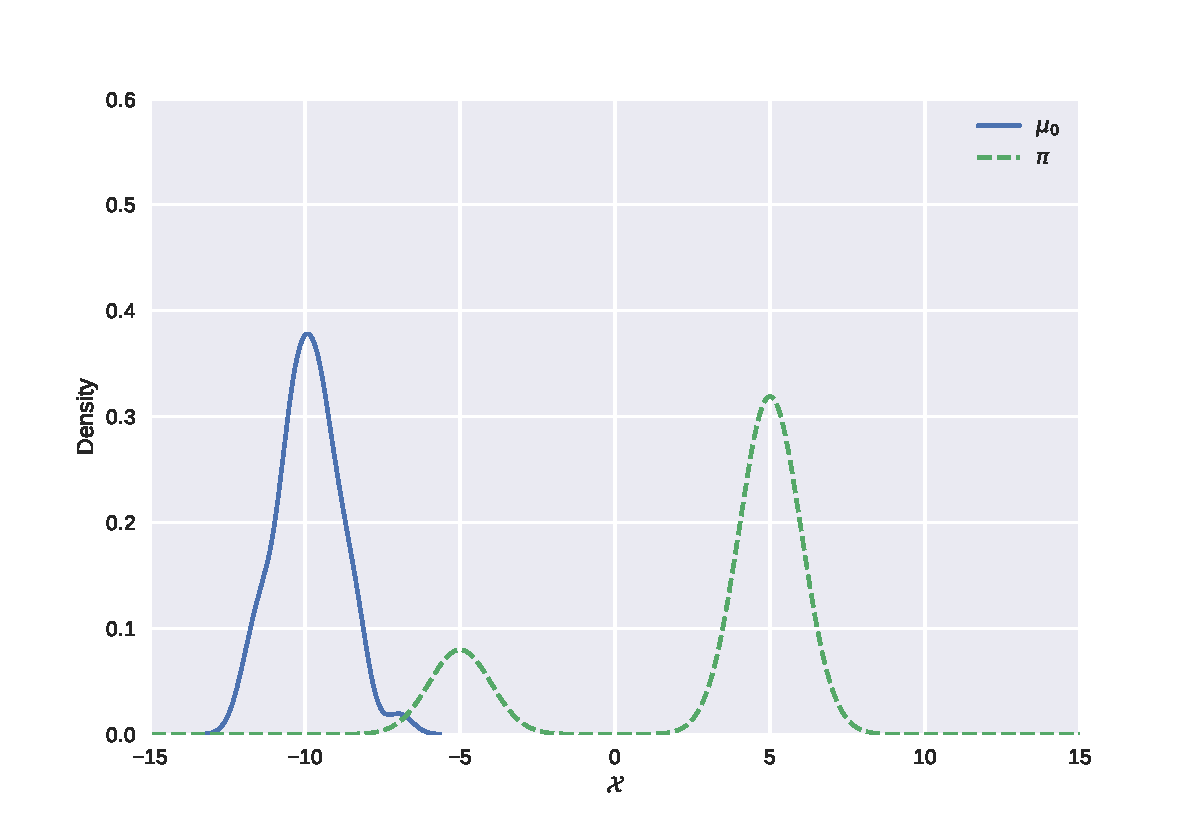
\includegraphics[width=\textwidth]{exp1-0.pdf}
    \caption{Iteration 1}
  \end{subfigure}
  \begin{subfigure}{0.32\textwidth}
    \centering
    \includegraphics[width=\textwidth]{exp1-100.pdf}
    \caption{Iteration 100}
  \end{subfigure}
  \begin{subfigure}{0.32\textwidth}
    \centering
    \includegraphics[width=\textwidth]{exp1-500.pdf}
    \caption{Iteration 500}
  \end{subfigure}

  \caption{Several iterations of the SVGD algorithm
    of the first experiment. One can see that the
    algorithm get stuck in a local minimum, making $\hat{\mu}_t$
    only follow the first modes of $\pi$.}
  \label{fig:exp1}
\end{figure}

\begin{figure}[H]
  \centering
  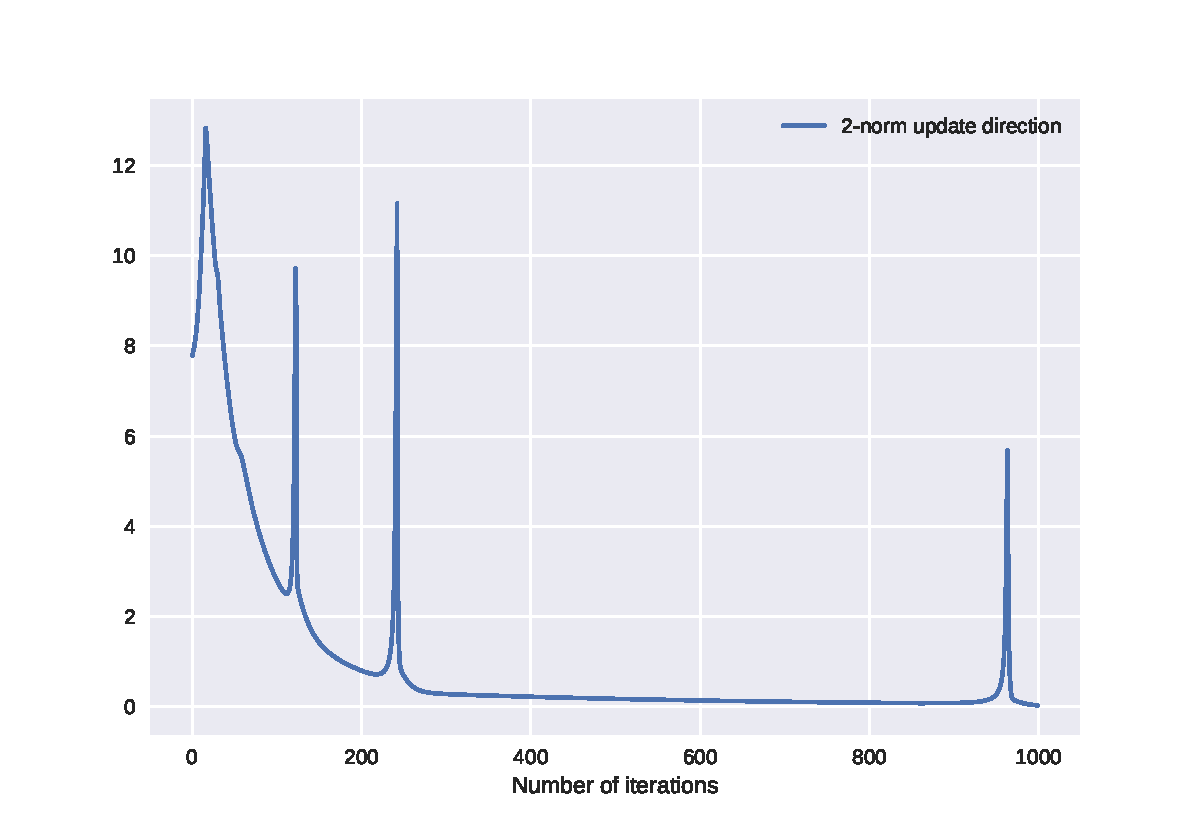
\includegraphics[width=0.6\textwidth]{norm_direction.pdf}
  \caption{2-norm of the update direction of the particles
    for the first experiment. It corroborates the fact that
    the algorithm get stuck in a local minimum.}
  \label{fig:norm-update}
\end{figure}

\begin{figure}[H]
  \centering
  \includegraphics[width=0.6\textwidth]{KL-exp1.pdf}
  \caption{Exponential decrease of the $\KL$ divergence
    over time for the first experiment. $\lambda=0.01$.}
  \label{fig:KL-exp1}
\end{figure}

\begin{figure}[H]
  \centering
  \begin{subfigure}{0.32\textwidth}
    \centering
    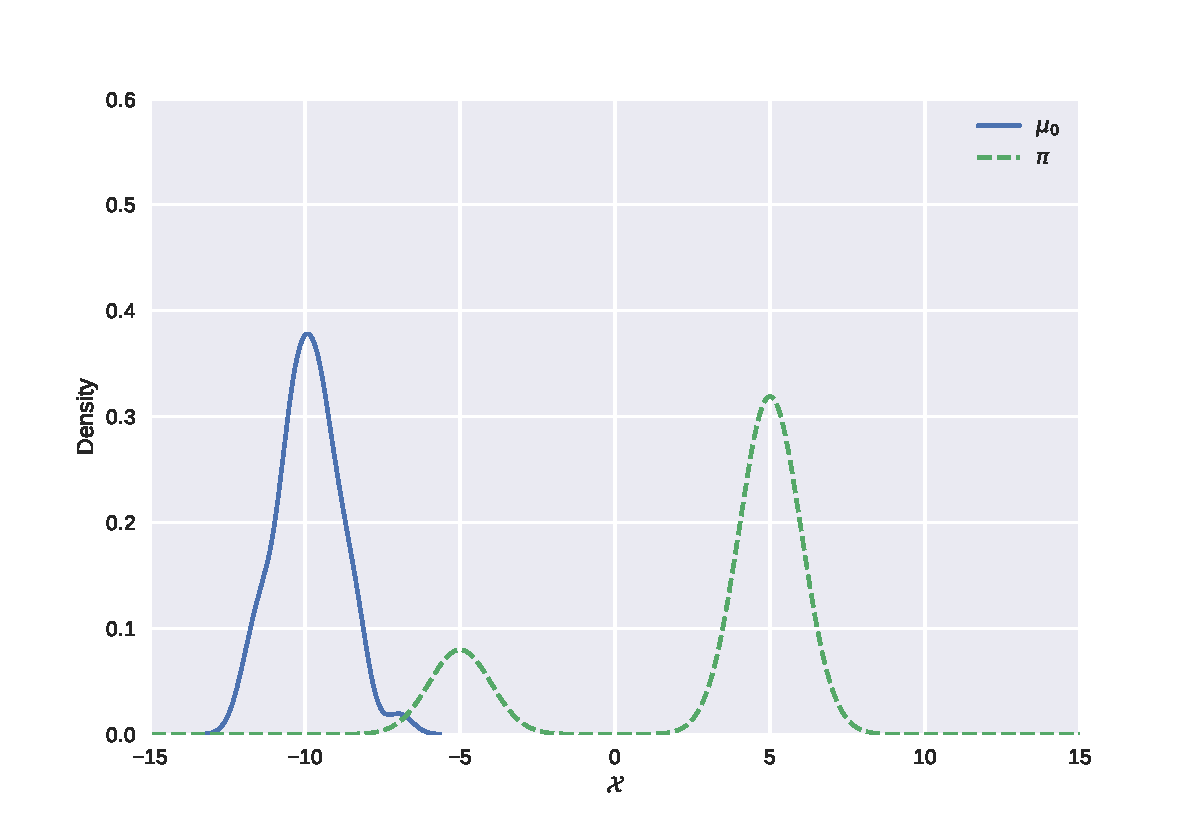
\includegraphics[width=\textwidth]{exp1-0.pdf}
    \caption{Iteration 1}
  \end{subfigure}
  \begin{subfigure}{0.32\textwidth}
    \centering
    \includegraphics[width=\textwidth]{exp1-100.pdf}
    \caption{Iteration 100}
  \end{subfigure}
  \begin{subfigure}{0.32\textwidth}
    \centering
    \includegraphics[width=\textwidth]{exp1-500.pdf}
    \caption{Iteration 500}
  \end{subfigure}

  \caption{Several iterations of the SVGD algorithm
    of the second experiment. One can see that the
    algorithm is able to take into account both modes of $\pi$.}
  \label{fig:exp2}
\end{figure}

\begin{figure}[H]
  \centering
  \includegraphics[width=0.6\textwidth]{KL-exp1.pdf}
  \caption{Exponential decrease of the $\KL$ divergence
    over time for the second experiment. $\lambda=0.001$.}
  \label{fig:KL-exp2}
\end{figure}

\section{Discussions}

\section{Conclusion}


\bibliographystyle{plainnat}
\bibliography{biblio}

\appendix
\section{Proofs}
\subsection{Proof of \ref{eq:stein_id}}
\begin{proof}\label{proof:stein_id}
  \begin{align*}
    \E_{x \sim \mu}[\A_\mu \phi (x)] &=
      \int_\X \pare*{ \nabla \log \mu(\cdot)^\top \phi(\cdot) + \nabla \cdot \phi(\cdot) } \mu(x) \d x \\
    &= \int_\X \nabla \log \mu(\cdot)^\top \phi(\cdot) \mu(x) \d x + \int_\X \nabla \cdot \phi(\cdot) \mu(x) \d x \\
    &= \int_\X \nabla \log \mu(\cdot)^\top \phi(\cdot) \mu(x) \d x +
      \int_\X \sum_{k=1}^d \diff{\phi_k}{x_k} \mu(x) \d x \\
    &= \int_\X \nabla \log \mu(\cdot)^\top \phi(\cdot) \mu(x) \d x +
    \sum_{k=1}^d \pare*{\int_{\partial X}\pare*{\pi(x) \phi_k(x)} \cdot n \d n - \int_\X \diff{\mu(x)}{x_k} \phi_k(x) \d x} \\
    &= \int_\X \nabla \log \mu(\cdot)^\top \phi(\cdot) \mu(x) \d x -
      \int_\X \sum_{k=1}^d \diff{\mu(x)}{x_k} \phi_k(x) \d x \\
    &= \int_\X  \mu(x) \sum_{k=1}^d \diff{\log \mu(x)}{x_k}\phi_k(x) -
    \mu(x) \sum_{k=1}^d \diff{\log \mu(x)}{x_k} \phi_k(x) \d x \;\; \text{(log trick)} \\
    &= 0
  \end{align*}
\end{proof}
\subsection{Proof of \ref{eq:stein_ksd_sol}}
\begin{proof}\label{proof:KSD}
  We first need to prove that
  $$
  \E_{x \sim \mu} \sq*{ \A_\pi f(x) } = \sca*{f, \phi^*}_\H, \; \forall f \in \H:
  $$
  \begin{equation*}
    \begin{split}
      \sca*{f, \phi^*}_\H &= \sum_{l=1}^d \sca*{ f^{(l)},
        \E_{x \sim \mu}\sq*{ k(x, \cdot) \nabla \log \pi(x)^{(l)} + \nabla k(x, \cdot)^{(l)}} }_{\H^0} \\
        &= \E_{x \sim \mu}\sq*{ \sum_{l=1}^d \sca*{f^{(l)}, k(x, \cdot)
          \nabla \log \pi(x)^{(l)} + \nabla k(x, \cdot)^{(l)} }_{\H^0} } \\
        &= \E_{x \sim \mu}\sq*{ \sum_{l=1}^d \nabla \log \pi(x)^{(l)}
          \sca*{ f^{(l)}, k(x, \cdot) }_{\H^0} + \sca*{ f^{(l)}, \nabla k(x, \cdot)^{(l)} }_{\H^0} } \\
        &= \E_{x \sim \mu}\sq*{ \sum_{l=1}^d \nabla \log \pi(x)^{(l)} f^{(l)}(x) + \nabla_{x_l} f(x)^{(l)} }
         \text{ (see \cite{Zhou2008}) } \\
        &= \E_{x \sim \mu}\sq*{ \nabla \log \pi(x)^\top f(x) + \nabla \cdot f(x) } \\
        &= \E_{x \sim \mu} \sq*{ \A_\pi f(x) }.
    \end{split}
  \end{equation*}
  Moreover, $\sca*{ f, \phi* }_\H \leq \norm{f}_\H \norm{\phi^*}_\H$.
  Thus,
  $$
  \S(\mu, \pi) =
    \max_{f \in \H} \bra*{ \E_{x \sim \mu}[\A_\pi f (x)] = \sca*{f, \phi^*}_\H, \; s.t. \; \|f\|_{\H} \leq 1 }
    \leq \norm{\phi^*}_\H.
  $$
  Let $f = \frac{\phi^*}{\norm{\phi^*}_\H}$, then $\norm{f}_\H = 1$ and
  $$
  \E_{x \sim \mu}[\A_\pi \phi (x)] = \sca*{f, \phi^*}_\H = \norm{\phi^*}_\H,
  $$
  ending the proof.
\end{proof}
\subsection{Proof that $\E_{x \sim \mu}[\A_\pi \phi (x)]$ measures the disperancy between $\mu$ and $\pi$}
\begin{proof}\label{proof:Esp_distance}
    \begin{equation*}
  \begin{split}
    \E_{x \sim \mu}[\A_\pi \phi (x)] &=
      \int_\X \pare*{ \nabla \log \pi(x)^\top \phi(x) + \nabla \cdot \phi(x) } \mu(x) \d x \\
    &= \int_\X \nabla \log \pi(x)^\top \phi(x) \mu(x) \d x +
    \sum_{k=1}^d \pare*{ \mathcal{R}_k - \int_\X \diff{\mu(x)}{x_k} \phi_k(x) \d x} \\
    &= \sum_{k=1}^d \mathcal{R}_k +
      \int_\X  \mu(x) \sum_{k=1}^d \diff{\log \pi(x)}{x_k}\phi_k(x) -
    \mu(x) \sum_{k=1}^d \diff{\log \mu(x)}{x_k} \phi_k(x) \d x \;\; \text{(log trick)} \\
    &= \sum_{k=1}^d \mathcal{R}_k +
      \sum_{k=1}^d \sq*{\mu(x) \phi_k(x)}_\X + \int_\X  \mu(x) \sq*{ \sum_{k=1}^d \phi_k(x) \pare*{ \diff{\log \pi(x)}{x_k} - \diff{\log \mu(x)}{x_k}}} \d x \\
    &= \sum_{k=1}^d \mathcal{R}_k +
      \sum_{k=1}^d \sq*{\mu(x) \phi_k(x)}_\X + \int_\X  \mu(x) \sq*{ \sum_{k=1}^d \phi_k(x) \pare*{ \diff{\log \frac{\pi(x)}{\mu(x)}}{x_k}}} \d x,
  \end{split}
\end{equation*}
\end{proof}

\subsection{Proof of $\H \subset L^2(\mu)$ (\ref{def:S-mu})}\label{pro:H-L2}
\begin{proof}
  We want to prove that, $\forall f \in \H$, 
  $\forall \mu \in \P_2(\X)$, $\int_\X f(x)^2 \d \mu(x) < \infty$.
  \begin{align*}
    \int_\X f(x)^2 \d \mu(x) &= \int_\X \sum_{l=1}^d \sca*{ f^{(l)}, k(x, \cdot) }^2_{\H_0} \d \mu(x) \\
    &\leq \sum_{l=1}^d \int_\X \norm*{f^{(l)}}^2_{\H_0} \norm*{k(x, \cdot)}^2_{\H_0} \d \mu(x)
      \text{ (by C.S)} \\
    &= \sum_{l=1}^d \norm*{f^{(l)}}^2_{\H_0} \int_\X \norm*{k(x, \cdot)}^2_{\H_0} \d \mu(x) \\
    &= \sum_{l=1}^d \norm*{f^{(l)}}^2_{\H_0} \int_\X \sca*{k(x, \cdot), k(x, \cdot)}_{\H_0} \d \mu(x) \\
    &= \sum_{l=1}^d \norm*{f^{(l)}}^2_{\H_0} \int_\X k(x, x) \d \mu(x)
      \text{ (by reproducing propriety)} \\
    &< \infty \text{, as } \int_\X k(x, x) \d \mu(x) < \infty.
  \end{align*}
\end{proof}

\subsection{Proof of \ref{eq:phi-Smu}}\label{pro:phi-Smu}
\begin{proof}
    Let $k$ in the Stein class of $\mu$. Thus:
    \begin{equation}
      \begin{split}
        P_\mu \nabla \log \frac{\mu}{\pi} (\cdot) &=
          \int_\X k(x, \cdot) \nabla \log \mu(x) \d \mu(x) - \int_\X k(x, \cdot) \nabla \log \pi (x) \d \mu(x) \\
        &= \int_\X k(x, \cdot) \nabla \mu(x) \d x - \int_\X k(x, \cdot) \nabla \log \pi (x) \d \mu(x) \\
        &= - \int_\X \nabla k(x, \cdot) \d \mu(x) - \int_\X k(x, \cdot) \nabla \log \pi (x) \d \mu(x) \\
        &= - \int_\X k(x, \cdot) \nabla \log \pi (x) + \nabla k(x, \cdot) \d \mu(x) \\
        &= -\phi^*(\cdot).
      \end{split}
    \end{equation}
\end{proof}

\subsection{Proof of Proposition \ref{prop:KL-Stein}}\label{pro:KL-Stein}
\begin{proof}
  The time derivative of the KL writes:
  \begin{align*}
    \diff{KL(\mu_t \| \pi)}{t} &= \diff{ }{t} \int_\X \log \frac{\mu_t(x)}{\pi(x)} \d \mu_t(x) \\
    &= \int_\X \diff{\mu_t(x)}{t} \log \frac{\mu_t(x)}{\pi(x)} \d x
      + \int_\X \mu_t(x) \diff{\log \frac{\mu_t(x)}{\pi(x)}}{t} \d x \\
    &= \int_\X \diff{\mu_t(x)}{t} \log \frac{\mu_t(x)}{\pi(x)} \d x
      + \int_\X \mu_t(x) \diff{\log \mu_t(x)}{t} \d x \\
    &= \int_\X \diff{\mu_t(x)}{t} \log \frac{\mu_t(x)}{\pi(x)} \d x
      + \int_\X \mu_t(x) \frac{\diff{\mu_t(x)}{t}}{\mu_t(x)} \d x \\
    &= \int_\X \diff{\mu_t(x)}{t} \log \frac{\mu_t(x)}{\pi(x)} \d x
      + \int_\X \diff{\mu_t(x)}{t} \d x \\
    &= \int_\X \diff{\mu_t(x)}{t} \log \frac{\mu_t(x)}{\pi(x)} \d x
   , \pare*{\text{ $\mu_t$ is a probability measure, so } \forall t, \int_\X \d \mu_t(x) = 1}
  \end{align*}
  Furthermore, as $\mu_t$ satisfies the continuity equation~(\eqref{def:continuity-equation})
  where $v_t = -P_{\mu_t} \nabla \log \frac{\mu}{\pi}$, we have:
  \begin{align*}
    \diff{KL(\mu_t \| \pi)}{t} &= -\int_\X \nabla \cdot (\mu_t(x) v_t(x)) \log \frac{\mu_t(x)}{\pi(x)} \d x \\
    &= -\sum_{l=1}^d \int_\X \diff{\mu_t(x) v_t(x)}{x_l} \log \frac{\mu_t(x)}{\pi(x)} \d x \\
    &= -\int_{\partial X} \pare* {\mu_t(x) v_t(x) \log \frac{\mu_t(x)}{\pi(x)}} \cdot n \d n
      + \sum_{l=1}^d \int_\X \mu_t(x) v_t(x) \diff{\log \frac{\mu_t(x)}{\pi(x)}}{x_l} \d x \\
    \text{The first term cancels }& \text{as probability densities tends to zero on the boundary.} \\
    &= \int_\X v_t(x) \nabla \log \frac{\mu_t(x)}{\pi(x)} \d \mu_t(x) \\
    &= \sca*{v_t, \nabla \log \frac{\mu_t}{\pi}}_{L^2(\mu_t)} \\
    &= \sca*{\iota^* v_t, \iota^* \nabla \log \frac{\mu_t}{\pi}}_{\H} \\
    &= \sca*{-\iota^* \iota S_{\mu_t} \nabla \log \frac{\mu_t}{\pi}, S_{\mu_t} \nabla \log \frac{\mu_t}{\pi}}_{\H} \\
    &= -\norm*{S_{\mu_t} \nabla \log \frac{\mu_t}{\pi}}_\H^2
  \end{align*}
\end{proof}

\subsection{Proof of \ref{eq:exp-KL}}\label{pro:exp-KL}
\begin{proof}
  Assume that $\pi$ satisfies the Stein log-Sobolev inequality.
  We have
  \begin{align*}
    \KL(\mu_t || \pi) &\leq \frac{1}{2\lambda} I_{Stein}(\mu_t || \pi)\\
    -I_{Stein}(\mu_t || \pi) &\leq -2\lambda \KL(\mu_t || \pi).
  \end{align*}
  Now, using Proposition~\ref{prop:KL-Stein}:
  \begin{align*}
    \diff{\KL(\mu_t || \pi)}{t} &\leq -2\lambda \KL(\mu_t || \pi) \\
    \KL(\mu_t || \pi) &\leq \KL(\mu_0 || \pi) \exp \pare*{ \int_0^t -2 \lambda \d s }
    \text{ (Gronwall's lemma) } \\
    \KL(\mu_t || \pi) &\leq e^{-2\lambda t} \KL(\mu_0 || \pi)
  \end{align*}
    
\end{proof}

\end{document} 
